\documentclass[12pt, twoside]{article}
\usepackage{jmlda}
\usepackage{amsfonts}
%\usepackage{algorithm}
%\usepackage{algcompatible}
\usepackage{algorithmic}
\usepackage{booktabs,siunitx}
\usepackage{bm}
\usepackage[outline]{contour}
%\usepackage{slashbox}
\usepackage{diagbox}

\usepackage{varwidth}
%\usepackage[figuresright]{rotating}
\usepackage[figuresleft]{rotating}
\usepackage{tabularx}
\usepackage{ragged2e}
\usepackage{lipsum}% for dummy text
%\usepackage[showframe]{geometry}

\graphicspath{{../figures/}}
\raggedbottom
\usepackage{float}

%\usepackage{caption}
%\captionsetup{justification=justified}
\usepackage{boxhandler}

\usepackage{algorithm}
\usepackage{lipsum}

\makeatletter
\newenvironment{breakablealgorithm}
  {
   \begin{center}
     \refstepcounter{algorithm}% New algorithm
     \hrule height.8pt depth0pt \kern2pt% \@fs@pre for \@fs@ruled
     \renewcommand{\caption}[2][\relax]{% Make a new \caption
       {\raggedright\textbf{\fname@algorithm~\thealgorithm} ##2\par}%
       \ifx\relax##1\relax % #1 is \relax
         \addcontentsline{loa}{algorithm}{\protect\numberline{\thealgorithm}##2}%
       \else % #1 is not \relax
         \addcontentsline{loa}{algorithm}{\protect\numberline{\thealgorithm}##1}%
       \fi
       \kern2pt\hrule\kern2pt
     }
  }{% \end{breakablealgorithm}
     \kern2pt\hrule\relax% \@fs@post for \@fs@ruled
   \end{center}
  }
\makeatother

%\usepackage{algpseudocode}
%\usepackage{array,calc}
%\usepackage{longtable,tabu}
%\usepackage{tabularray}
%\usepackage{caption}
%\usepackage{diagbox}
%\usepackage{multirow}
%\newlength{\dig}
%\settowidth{\dig}{6}


\renewcommand{\thealgorithm}{}

\newcommand{\hdir}{.}



\begin{document}

\English

\title
    [] % short title for page headings, not necessary if a full title fits the headings
    {Influence of hyperparameters on online aggregation with countable experts} % full title
\author
    [S.\,M.~Kunin-Bogoiavlenskii] % short list of the authors (<= 3) for page headings, is necessary only if the full list does not fit the headings
%S.M. Kunin-Bogoiavlenskii, A.V. Zukhba, and R.D. Zukhba
    {S.\,M.~Kunin-Bogoiavlenskii, A.\,V.~Zukhba, R.\,D.~Zukhba, and V.\,V.~V’yugin} % full list of the authors, presented in the table of contetns of the issue
    [S.\,M.~Kunin-Bogoiavlenskii, A.\,V.~Zukhba, R.\,D.~Zukhba] % list of the authors presented in the title page of the article, is necessary only if it differs from the full list of the authors in braces, i.e. '{' and '}'
\email
    {kunin-bogoiavlenskii.sm@phystech.edu; a\_\_l@mail.ru; zukhba.rd@phystech.edu}
%\thanks
%    {The research was
%     %partially
%     supported by the Russian Foundation for Basic Research (grants 00-00-0000 and 00-00-00001).}
\organization
    {Moscow Insitute of Physics and Technology}
\abstract
    {

    Aggregating forecasts from multiple experts is a valuable method to improve prediction accuracy.
    This paper examines the influence of hyperparameters on the performance of the aggregation algorithm for a countable number of experts.
    We implement a time series generator with specified properties and an aggregating forecasting model. 
    We conduct a series of experiments with various hyperparameters of the algorithm (including initialization weights, mixing update coefficients, etc.), and propose a new mixing scheme, used in the algorithm.
    The experiments confirm that these hyperparameters have a significant influence on the algorithm's performance.           
        
%   \noindent
%   \textbf{Background}:    One paragraph about the problem, existent approaches and its limitations.
%   
%   \noindent
%   \textbf{Methods}: One paragraph about proposed method and its novelty.
%   
%   \noindent
%   \textbf{Results}: One paragraph about major properties of the proposed method and experiment results if applicable.
%   
%   \noindent
%   \textbf{Concluding Remarks}: One paragraph about the place of the proposed method among existent approaches.
%               
    \noindent
        \textbf{Keywords}: \emph{online learning; aggregating algorithm; prediction with experts’ advice; Fixed Share, Mixing Past Posteriors (MPP)}}

%these fields are filled in by the journal editors
%\doi{10.21469/22233792}
%\receivedRus{01.01.2017}
\receivedEng{January 01, 2017}

\maketitle
%\linenumbers

\section{Introduction}
%\noindent %this command is placed at the beginning of the first sentence of each paragraph/section only.
This work is inspired by the algorithm, developed in the article \cite{article}, considering online game of prediction with experts' advice. The data is presented as a time series, consisting of outcome pairs --- <<signal>> and <<response>>. 
In contrast to the classical statistical theory of sequential prediction, we make no assumptions about the nature of the data (which could be deterministic, stochastic, etc.). 
We use machine learning methods to build forecasters within a game-theoretic approach.
The online learning master model considers a series of reference forecasters, referred to as experts, to build its opinion by combining their predictions.


%\noindent
The general prediction algorithm with expert advice follows this structure:
Learning progresses in trials at discrete points in time. 
During each step , expert models, based on past observational data subsamples, provide their predictions. 
The master model then makes a decision using the chosen aggregating algorithm. 
At the end of the trial, the generator presents the true outcome, and both the master and expert models are scored using a loss function. 
The difference between the master's cumulative losses and the expert's cumulative losses is defined as regret.
The traditional goal of the aggregating algorithm is to keep it as small as possible.

%\noindent
We use special assumptions about the data generation structure when building forecasting strategies. 
It is assumed that there are multiple generators, whose structure is unknown to the predictors. 
The time series is obtained by merging segments, each produced by one of the generators. 
These segments are called areas of stationarity, and can be studied using machine learning methods.
%These generators switch, producing a time series that is subdivided into a sequence of segments --- areas of stationarity, which can be studied using machine learning methods. 
Each corresponding local predictive model will be constructed based on data from the area of stationarity and can be then successfully applied in other areas of stationarity generated by the same generator.

%\noindent
In this formulation of the forecasting problem, the series of prediction steps is divided into segments that frame arbitrary sequences of expert strategies. 
The sequence of segments and its associated sequence of experts is called a partition. 
The modified goal of the aggregating algorithm is to perform well relative to the best partition. 
Accordingly, the new concept of algorithm regret is the difference between the algorithm's losses and the cumulative losses of the sequence of experts. 
This change allows for a more accurate modeling of real-life conditions, where the nature of responses may change over time and different experts may predict with varying degrees of success depending on the current trend. 

%\noindent
The corresponding algorithm is called Fixed Share \cite{article98}. 
A further proposed generalization of it is the Mixing Past Posteriors (MPP) method \cite{article02}. 
%The cumulative losses of the aggregating algorithm are related to convex combinations of expert losses. 
%The concept of regret also changes. 
%Now the algorithm's cumulative losses are compared to the cumulative losses of convex combinations of expert strategies.
A characteristic feature of the problem considered in \cite{article} is the absence of a predefined set of competing expert strategies, as was the case in the works cited above.
Instead, new expert strategies are constructed at each step of the online learning process.
The master must aggregate the forecasts of all expert strategies constructed up to that time in real-time at each step. 
Algorithm GMPP, proposed in \cite{article}, is the foundation of our experiments. 

In our work, we systematically explore the impact of various hyperparameters on the algorithm, including different weight functions for initializing experts, 
various mixing schemes for combining expert predictions, and different update coefficient functions. 
We also analyze algorithm performance in situations of lack of information,  experimenting with different sizes of the expert training window and noise level in the data. 
We propose a new mixing scheme called <<Increasing Past Share>> that emphasizes older expert predictions, 
doing so more smoothly than the default scheme in the GMPP algorithm, which helps to incorporate more historical information.

\section{Problem statement}
%\paragraph{Definitions}
Let $x_1, x_2, \dots$ be the sequence of signals belonging to the sample space  $\mathcal{X}$. 
The masters goal is to predict the sequence of the corresponding responces $y_1, y_2, \dots$ belonging to the outcome space $\mathcal{Y}$. 
We assume that the master knows $a, b \in \RR$ --- the bounds of the responces sequence, s.t. $\forall i\quad a \leq y_i \leq b$.
There is a countable number of experts $i \in \mathcal{N}$, where $\mathcal{N}$ is the natural numbers set. 
%We assume that there is a countable number of experts $i \in \mathcal{N}$, where $\mathcal{N}$ is the natural numbers set. 
%The predictions of the master and experts also belong to $\mathcal{Y}$. 
Let $ \lambda: \mathcal{Y} \times \mathcal{Y} \rightarrow \RR_+$ be the nonnegative loss function. 

At each step $t$ every expert $i \in \mathcal{N}$ provides his prediction $f_t^i = f_t^i(x_t)  \in \mathcal{Y}$. 
After obtaining them the master gives his prediction $p_t = p_t(x_t) \in \mathcal{Y}$. 
Next, the generator reveals the true outcome $y_t$, and the losses are computed.
Let $h_t = \lambda(p_t, y_t)$ be the master's loss , and $l_t^i = \lambda(f_t^i, y_t)$ be the loss of expert $i \le t$. For $i > t$ (i.e. expert $i$ is not yet initialized), $l_t^i = h_t$.

With designations $L_T^i = \sum_{t = 1}^T l_t^i$, representing the cumulative loss of expert $i$ during the first T steps, and $H_T = \sum_{t = 1}^T h_t$, 
representing the master's cumulative loss during the first T steps, we can define the master's regret relative to the expert $i$ as $R^i_T = H_T - L^i_T$. 

The best partition is formed based on a hindsight analysis of the experiment results, assuming we know the segment boundaries. For each segment, the best partition predictions are set equal to the predictions of the best local expert (the one that has the lowest cumulative sum on that segment). Master's regret relative to the best partition is defined as $R_T= H_T - L_T$, where $L_T$ is the cumulative loss of the best partition. We use $R_T$ as a metric in our experiments.

 
%\paragraph{Aggregating algorithm}
\vspace{5mm}

\begin{breakablealgorithm}
\caption{GMPP}
\begin{algorithmic}
%\STATE Parameters:
%\STATE \textbullet~ Initialization weights $w^i_1$, s.t. $\sum\limits_{i \in \mathcal{N}}w^i_1 = 1$
%\STATE \textbullet~ Alpha parameter series $\{\alpha_t\}$
%\STATE \textbullet~ Train window size 

\STATE Initialize the weights $w^i_1$ so that $\sum\limits_{i \in \mathcal{N}}w^i_1 = 1$
\FOR{$t = 1, 2, \dots$}

  
\STATE\textbf{\textperiodcentered}~ Expert $f^t$ initialization
\STATE\textbf{\textperiodcentered}~ Signal $x_t$ is received 
\STATE\textbf{\textperiodcentered}~ Experts' predictions $f_t^i = f_t^i(x_t), 1 \le i \le t$ 
\STATE\textbf{\textperiodcentered}~ Computation of normalized weights of experts  $1 \le i \le t$: $\widehat{w}^i_t = \dfrac{w^i_t}{\sum_{j=1}^t w_t^j}$
\STATE\textbf{\textperiodcentered}~ Master's prediction evaluation $\gamma_t = \textit{Subst}(\mathbf{f_t}, \mathbf{\widehat{w}_t}) = \dfrac{a+b}{2} + \dfrac{1}{2\eta(b-a)}\cdot \ln \dfrac{\sum\limits_{i \in \mathcal{N}} \hat w_t^i e^{-\eta(b - f_i)^2}}{\sum\limits_{i \in \mathcal{N}}  \hat w_t^i e^{-\eta(a - f_i)^2}}$, \\ where $\mathbf{\widehat{w}_t} = (\widehat{w}_t^1, \widehat{w}_t^2, \dots \widehat{w}_t^t),\ \mathbf{f_t} = (f_t^1, f_t^2, \dots f_t^t)$
\STATE\textbf{\textperiodcentered}~ True outcome $y_t$ is revealed
\STATE\textbf{\textperiodcentered}~ Computation of master's loss $h_t = \lambda(p_t, y_t) $ and experts' losses: $l_t^i =
\begin{cases}
        \lambda(f_t^i, y_t), & \text{if $i \le t$} \\
        h_t, & \text{if $i > t$}
\end{cases}$
\STATE\textbf{\textperiodcentered}~ \textbf{Loss Update} weights modification
\[  \widetilde{w}_t^i = \dfrac{w_t^i e^{\eta l_t^i}}{\sum\limits_{j = 1}^t w_t^j e^{-\eta l_t^i} + e^{-\eta h_t} (1 - \sum\limits_{j = 1}^t w_t^j) } \]
\STATE\textbf{\textperiodcentered}~ \textbf{Mixing Update} weights modification
\[  \widetilde{w}_{t+1}^i = \alpha_t\widetilde{w}_1^i + (1 - \alpha_t)\widetilde{w}_t^i\] 

\ENDFOR


\end{algorithmic}
\end{breakablealgorithm} 

\section{Experiment}
We implement the synthetic time series generator and the GMPP algorithm itself. 
We then conduct experiments to analyze the effects of varying hyperparameters.
As can be seen from the algorithm, the time computational complexity of the algothim is quadratic. 
Therefore , we fix certain length of time series for all experiments.
\subsection{Data generation}

We define generators $G_1, G_2, \dots, G_k$ by their weight vectors $\vec w_1, \vec w_2, \dots, \vec w_k \in \RR^d$. 
Here, $d$ represents the dimensionality of the signals.

We generate signals as a series of vectors $\vec x_1, \vec x_2, \dots, \vec x_T \sim \mathcal{N}(0, I_d)$, indicating they are drawn from a zero-mean Gaussian distribution with an identity covariance matrix .
%We randomly divide this sequence of vectors into a series of segments.
%%This series of vectors is then randomly divided into a sequence of segments. 
%We denote these segments as $S_1, S_2, \dots, S_m$. 
%Each segment $S_i$ is a sequence of vectors itself, containing elements from $\vec x_{s_{i-1}+1}$ to $\vec x_{s_i}$ (where $s_i$ is the index of the last element in segment $i$, $s_0 = 0$). 
We randomly divide this sequence of vectors into a series of segments $\{S_1, S_2, \dots, S_m\}$ = $\{\{ \vec x_1, \vec x_2, \dots, \vec x_{|S_1|}\}, \{\vec x_{|S_1|+1}, \vec x_{|S_1|+2}, \dots, \vec x_{|S_1| + |S_2|}\}, \dots, \{\vec x_{T-|S_m|+1}, \vec x_{T-|S_m|+2}, \dots, \vec x_{T}\}\}$. 
Importantly, each segment $S_i$ corresponds to a specific generator $G_{g(i)}$ according to a random function $g$. 
This function determines which generator is responsible for creating responses for that segment. In our experiment, $g(i)$ is uniformly distributed in $\{1, 2, \dots, k\} \backslash \{g(i-1)\}$, so adjacent segments correspond to different generators.

Ultimately, we obtain the series of responses $y_1, y_2, \dots, y_T$ by taking the dot product of each signal vector with the weight vector of the corresponding  generator and adding the noise: $y_i = \langle \vec w_{g(i)}, \vec x_i \rangle + \varepsilon_i,$ where $\varepsilon_i \sim \mathcal{N}(0, \sigma^2)$. If $y_i  \notin [a, b]$, we regenerate $x_i$ until this condition is met. For our properties, bootstrap shows this happens less than in $4\%$ of the cases, so can be considered insignificant.
\vspace{2mm}

In our experiment, we fix the following data characteristics:
\begin{itemize}
\item Time series length $T = 2000$,
\item Signals dimention $d=10$,
\item Generator weight vectors are drawn from a uniform distribution $U_{[-10, 10]^d}$,
\item Responses bounds $[a, b] = [-40, 40]$,
\item $|S_1|, |S_2|, |S_{m-1}|$ are drawn from a uniform distribution $U_{[50, 300]}$, and $|S_m| = T-\sum_{i=1}^{m-1}|S_i|$
\item Number of generators $k = 5$,
\item White noise variance $\sigma^2= 1$
\end{itemize}

Also, to ensure robust performance from the outset, we insert a short priming sequence at the beginning of the time series. 
This sequence includes one segment from each generator, sizes of segments are also drawn from  $U_{[50, 300]}$.
 Importantly, the data from this priming sequence is not included in the regret calculation. 
 Without such a sequence, losses in the beginning of the main series would be much higher than in general, which would deteriorate analysis of hyperparameters influence.
\subsection{Experts}

Each expert $f_t$ is initialized as a linear regression model. 
This model is trained on a fixed window of $l$ past observations. 
The training process yields a weight vector, which is calculated as  
$\theta_t = (\vec X^T\vec X)^{-1}\vec X^T\vec y$,\ where $\vec X^T = (\vec x_{t-1}, \vec x_{t-2}, \dots \vec x_{t-l}),\ \vec y = (y_{t-1}, y_{t-2}, \dots y_{t-l})$. 

Given a new signal vector  $\vec x$, the expert's prediction is obtained by calculating the dot product between the weight vector and the signal vector: $f_t(\vec x) = \langle \vec \theta_t, \vec x \rangle$ 

\subsection{Hyperparameters}

We investigate the impact of various hyperparameters on the GMPP algorithm's performance, focusing on initialization weights, mixing scheme, mixing update coefficients, and expert window size. 
\begin{enumerate}
\item Initialization Weights ($w_1^t$):
\begin{itemize}
\item Default: $w_1^t = \frac{1}{(t+1)\ln^2(t+1)}$
\item Experimental: 
\begin{itemize}
%\item $w_1^t = \frac{1}{e^t}$, exploring exponential decay as a common alternative.
\item $w_1^t = \frac{1}{(t+4)\ln(t+4)\ln^2\ln(t+4)}$, representing a slower decaying function.
\item $w_1^t = \frac{1}{t^\alpha}$, with $\alpha \in (1, 2]$, to analyze the impact of faster decay rates.
\item $w_1^t = \frac{1}{t^\alpha}$, with $\alpha \in (0, 1]$, to analyze the behavior with diverging weights.


\end{itemize}
\end{itemize}


\contourlength{0.1pt}

\item Mixing Update Coefficients ($\alpha_t$):
\begin{itemize}
\item Default: $\alpha_t = \frac{1}{t+1}$
\item Experimental: 
\begin{itemize}
\item $\alpha_t = \frac{1}{(t+1)^\beta}$, with $\beta \in (0, 2]$, to analyze different decay speeds.
\item $\alpha_t = \frac{1}{t+c}$, with varying $c$, to analyze the influence of a constant shift.
\item $\alpha_t = \frac{1}{c}$, with $100 \le c \le10000$
\item $\alpha_t = \frac{1}{e^{t/3}}$, exponential decay.         

\end{itemize}


\end{itemize}

\item Mixing Update Scheme:

While GMPP in \cite{vvbook} utilizes a specific scheme, we explore various Mixing Fixed-Share Update schemes as presented in \cite{article02}:

\[ \widetilde{w}_{t+1}^i = \sum_{q=1}^t\beta_t(q)\widetilde{w}_q^i  \]

\begin{itemize}
\item Start Vector Share (default in GMPP) --- emphasizes the initial and the most recent  weight  vectors:
    \[\beta_t(q) =
    \begin{cases}
    \alpha_t, & q = 1 \\
    0, & 1 < q < t \\
    1 - \alpha_t, & q = t 
    \end{cases}\]
    
\item Uniform Past Share ---  assigns equal weight to all past weight vectors : 
    \[\beta_t(q) =
    \begin{cases}
    \alpha_t\frac{1}{t}, & 1 \le q < t \\
    1 - \alpha_t, & q = t 
    \end{cases}\]
    
\item Decaying Past Share ---  assigns decreasing weights to past weight vectors:
    \[\beta_t(q) =
    \begin{cases}
    \alpha_t\frac{1}{(t-q)^\gamma}\frac{1}{Z_t}, & 1 \le q < t \\
    1 - \alpha_t, & q = t
    \end{cases}\]
    \hfill ,with $Z_t = \sum_{q=1}^{t-1} \frac{1}{(t-q)^\gamma}, \gamma > 0$. 
        
\end{itemize}

We also propose a new mixing scheme:
\begin{itemize}

\item Increasing Past Share --- assigns increasing weights to past weight vectors:
    \[\beta_t(q) =
    \begin{cases}
    \alpha_t(t-q)^\gamma\frac{1}{Z_t}, & 1 \le q < t \\
    1 - \alpha_t, & q = t
    \end{cases}\]
    \hfill ,with $Z_t = \sum_{q=1}^{t-1}(t-q)^\gamma, \gamma > 0$. 
        
\end{itemize}


\item Window Size ($l$): We vary train window size $l \in \{5, 10, 20, 50, 100\}$ to check algorithm performance in situations when experts lack information or when they often train on pieces made by different generators.

\end{enumerate}
%
%As a metric of quality we use $R_T$ --- master's regret relative to the best partition.
%We run experiments 4 times for each configuration of hyperparameters, and take the mean of the earned regrets.
%
%\newpage
\section{Results}

We analyze the impact of various hyperparameters on the GMPP algorithm's performance, focusing on initialization weights, mixing schemes, mixing update coefficients, and expert window size. Our primary performance metric is the mean regret relative to the best partition, calculated from four independent runs for each hyperparameter configuration.

\subsection{Impact of Initialization Weights}
Table \ref{table:mt_wf} explores the influence of different ways of initializing the weights of experts (the importance assigned to each expert at the start of the algorithm) on the regret. We highlight the lowest regret values in bold.


The results show that the best weight function can depend on the mixing scheme chosen. For example, in default scheme <<Start Vector Share>> weight functions based on diverging series yielded lower regret than those based on converging series. In this case, the $1/x^{0.5}$ weight function achieved the best performance (see Figure \ref{fig:diff_wf}). When employing converging weight series, schemes <<Increasing Past Share>> and <<Uniform Past Share>> appear to be better than others.



\begin{figure}[H]
\centering % <-- added
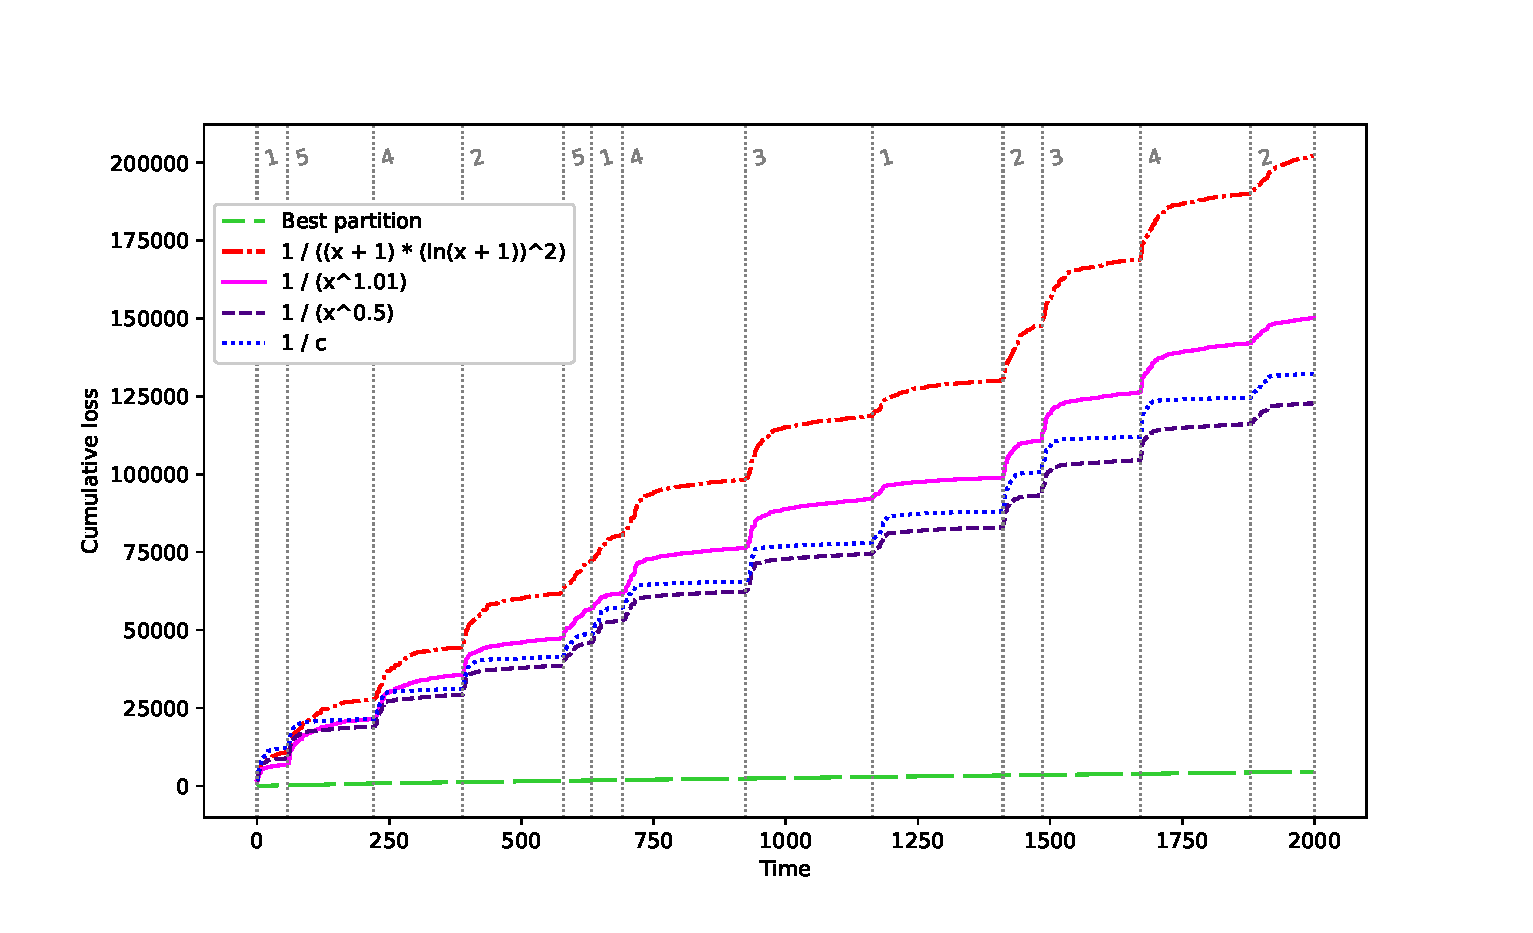
\includegraphics[width=1\linewidth]{diff_wf_styled}
\caption{\begin{varwidth}[t]{\linewidth}\centering Total loss for different weight functions \\(alpha function is defaut, $\sigma^2 =1$, window size = 10)\end{varwidth} \label{fig:diff_wf}}

\end{figure}


\begin{table}[H]
\centering
%\caption{Regret with different weight functions and mixing types}
\begin{tabular}{c|cccc}
\toprule
 & \multicolumn{4}{c}{Mixing Type} \\
\midrule
Weight Function & Decaying Past & Increasing Past & Start & Uniform Past \\
\midrule
$1 / ((x + 1)\ln^2(x + 1))$ & 122513.26 & 122383.91 & 175594.64 & 117175.93 \\
$1 / c$ & 128114.78 & 117241.85 & 113998.26 & 119703.68 \\
$1 / (x^{0.1})$ & 127435.12 & 115101.52 & 111276.08 & 117830.57 \\
$1 / (x^{0.3})$ & 126769.51 & 112900.36 & \contour{black}{108946.40} & 115819.07 \\
$1 / (x^{0.5})$ & 126191.99 & 111221.38 & \contour{black}{108630.68} & 114153.63 \\
$1 / (x^{0.7})$ & 125352.96 & \contour{black}{109775.49} & 112027.20 & 112378.87 \\
$1 / (x^{0.9})$ & 123969.39 & \contour{black}{109408.73} & 122832.21 & \contour{black}{110783.66} \\
$1 / x$ & 122965.58 & \contour{black}{110376.37} & 131907.11 & \contour{black}{110486.71} \\
$1 / (x^{1.01})$ & 123066.72 & \contour{black}{110438.09} & 132268.30 & \contour{black}{110569.83} \\
$1 / (x^{1.1})$ & 123963.12 & \contour{black}{111050.44} & 135253.09 & 111366.88 \\
$1 / (x^{1.2})$ & 124846.17 & 111873.03 & 137976.99 & 112298.14 \\
$1 / (x^2)$ & 133051.62 & 124473.63 & 148080.01 & 123449.14 \\
$1 / ((x + 4) \ln(x + 4)\ln^2(\ln(x + 4)))$ & 121229.77 & 119413.95 & 169065.24 & 114823.76 \\

\bottomrule
\end{tabular}
\caption{\begin{varwidth}[t]{\linewidth}\centering Regret with different weight functions and mixing types  
\\(alpha function is defaut, $\sigma^2 =1$, window size = 10)\end{varwidth} \label{table:mt_wf}}

\end{table}

%--------------------------------------------------------------------------------------------------------------------

\subsection{Influence of Training Window Size}

\begin{table}[H]
\centering

\begin{tabular}{c|ccccc}
\toprule
& \multicolumn{4}{c}{Mixing scheme} \\
\toprule
{Train Window} & decaying past & increasing past & start & uniform past & \\
\midrule
5 & 140895.88 & 155163.20 & 186550.57 & 150308.76 \\
10 & 123066.72 & \contour{black}{110438.09} & 132268.30 & \contour{black}{110569.83} \\
20 & 163303.00 & 121289.12 & 125763.68 & 127764.22 \\
50 & 187007.96 & 132165.07 & 136397.74 & 139560.71 \\
100 & 195888.54 & 143925.39 & 148888.73 & 150253.75 \\
\bottomrule
\end{tabular}
\caption{\begin{varwidth}[t]{\linewidth}\centering Regret with different Mixing Update schemes and Train Windows  \\ (alpha function is defaut, weight function is $1/x^{1.01}$, $\sigma^2 =1$)\end{varwidth} \label{table:tw}}

\end{table}

Table \ref{table:tw}  shows that the performance of the GMPP algorithm is generally sensitive to the training window size.
The best performance is achieved with a window size of 10, suggesting that a balance between having enough past data to train a good model and not being too influenced by older, potentially irrelevant data is important.
The different mixing schemes show varying performance, with the default GMPP scheme <<Start Vector Share>> (which emphasizes initial and recent weights) showing higher regret compared to the other schemes. Best performance in the conditions of enough informatin (with train window $\geq 10$) shows <<Increasing Past Share>> scheme.

%--------------------------------------------------------------------------------------------------------------------

\subsection{Influence of Noise}
Table \ref{table:noise} investigates how the noise in the generated responses affects the regret of the algorithm.  
Surprisingly, as the noise level increases, the regret decreases, and at some point, it even becomes negative (see Figure \ref{fig:noises}). 
The reason of this is that with size of the window equal only to 10, high noise can dramatically deteriorate training of the linear regression, leading to huge mistakes of the experts. As a resut, the master algorithm outperforms the best partition.
% Interestingly, the point at which the regret becomes negative varies depending on the mixing scheme.

\begin{table}[H]
\centering

\begin{tabular}{c|ccccc}
\toprule
& \multicolumn{4}{c}{Mixing scheme} \\
\toprule
{Noise variance} & \centering decaying past & \centering increasing past & \centering start & \centering uniform past &  \\
\midrule
0.10 & 131348.25 & 114564.74 & 131578.01 & 115927.25 \\

1 & 123066.72 & 110438.09 & 132268.30 & 110569.83 \\
2 & 109753.81 & 105398.29 & 136043.26 & 103136.06 \\
5 & 76132.46 & 92343.75 & 144554.62 & 83630.45 \\
6 & 17155.14 & 89032.63 & 146382.86 & 25178.60 \\
7 & -18273.00 & 29417.82 & 144827.02 & -9208.74 \\
8 & -83796.21 & -13307.43 & 147510.57 & -55905.83 \\
%9 & -1292481.14 & -66578.18 & 111455.10 & -79922.70 \\
10 & -649917.41 & -120166.34 & 90089.56 & -377184.32 \\
%11 & -677350.84 & -553834.55 & -4217467.46 & -4977614.29 \\
12 & -828973.51 & -1123130.94 & -420588.94 & -1354731.42 \\
%13 & -1297340.06 & -1127803.13 & -184977.56 & -1365609.14 \\
%14 & -1529645.72 & -1265872.25 & -213233.53 & -1633244.28 \\
%15 & -1376777.17 & -1508510.73 & -1205600.59 & -1862352.43 \\
%20 & -8506756.45 & -9004436.41 & -8784588.25 & -9007978.86 \\
%50 & -12031878.44 & -14242897.85 & -4704221.50 & -14879230.26 \\
\bottomrule
\end{tabular}
\caption{\begin{varwidth}[t]{\linewidth}\centering Regret with different Mixing Update schemes and Noise Variance \\ (mixing scheme is default, alpha function is defaut, weight function is $1/x^{1.01}$, window size = 10)\end{varwidth} \label{table:noise}} 
\end{table}



%\newpage

\begin{figure}[htb]
    \centering % <-- added
\begin{subfigure}{0.49\textwidth}
  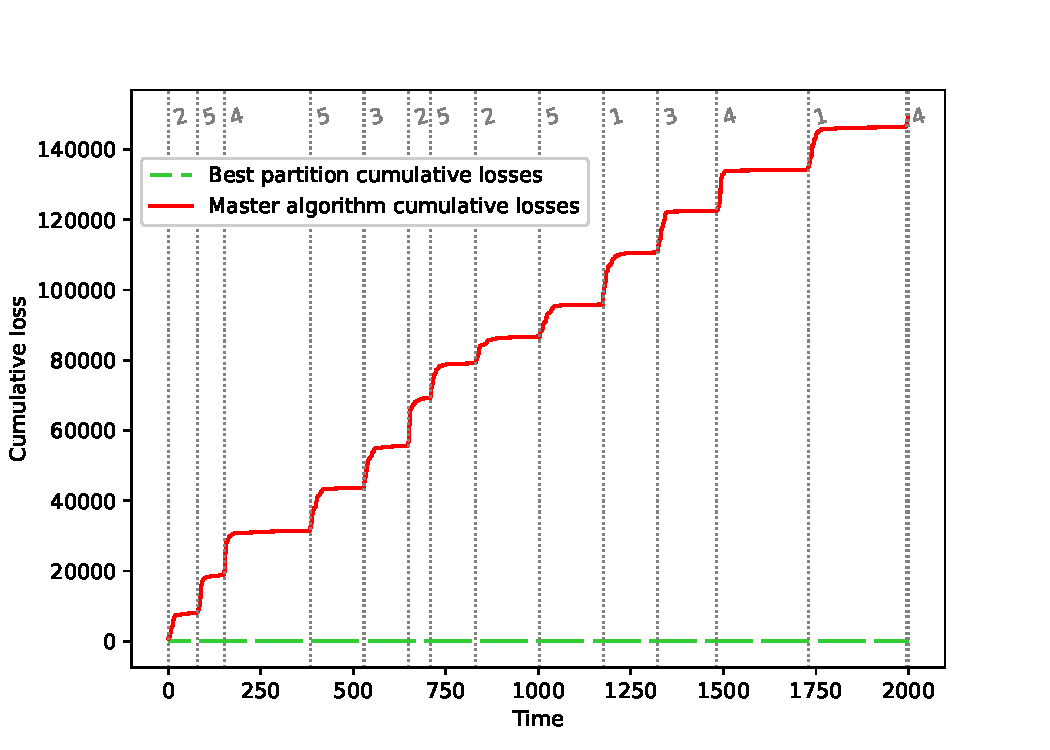
\includegraphics[width=\linewidth]{dec_noise_0.1}
  \caption{$\sigma^2$ = 0.1}
  \label{fig:n_1}
\end{subfigure}\hfil % <-- added
\begin{subfigure}{0.49\textwidth}
  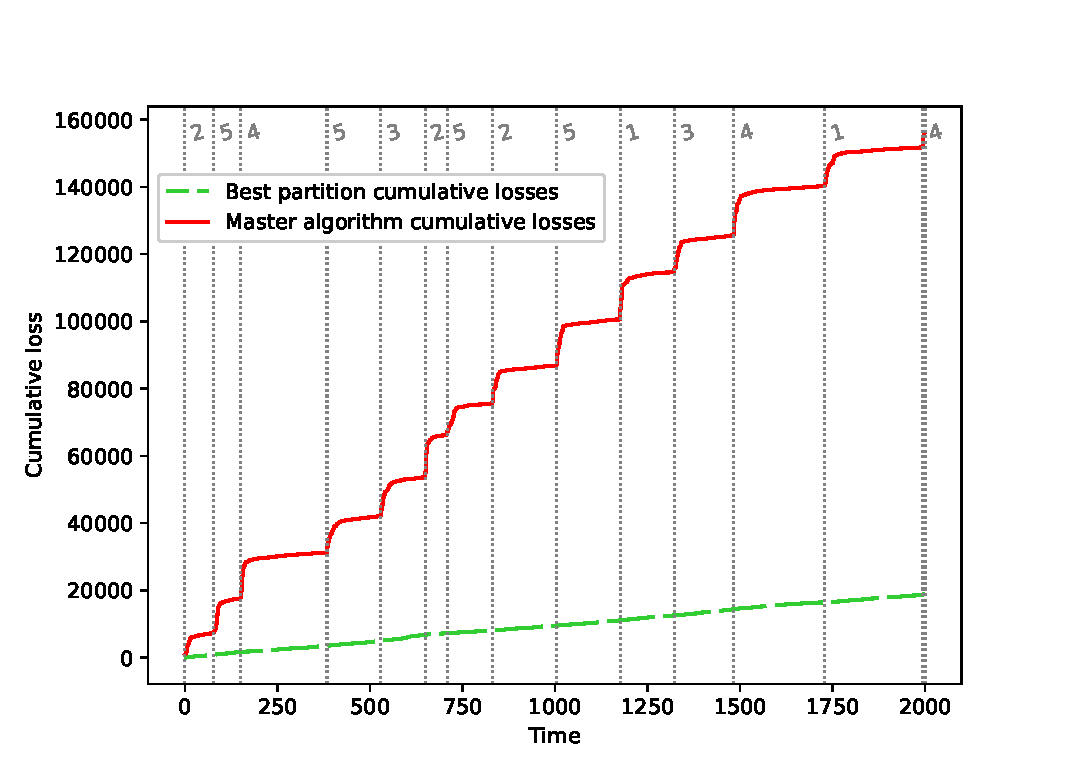
\includegraphics[width=\linewidth]{dec_noise_2}
  \caption{$\sigma^2$ = 2}
  \label{fig:n_2}
\end{subfigure}\hfil % <-- added

%\medskip
\begin{subfigure}{0.49\textwidth}
  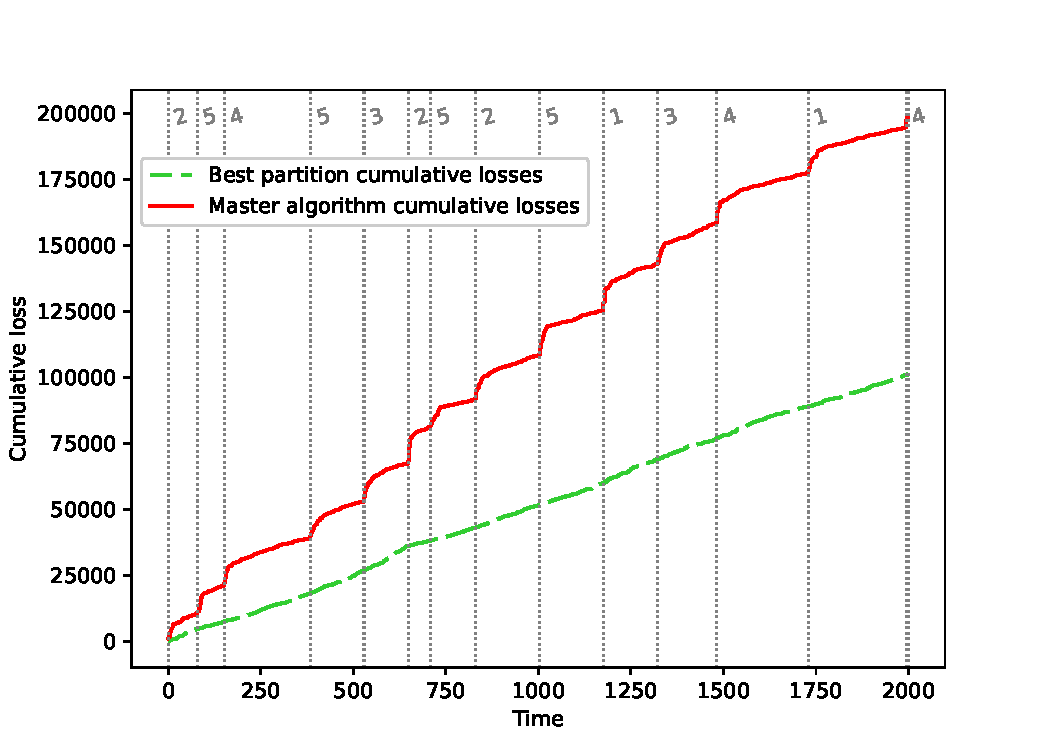
\includegraphics[width=\linewidth]{dec_noise_5}
  \caption{$\sigma^2$ = 5}
  \label{fig:n_5}
\end{subfigure}
\begin{subfigure}{0.49\textwidth}
  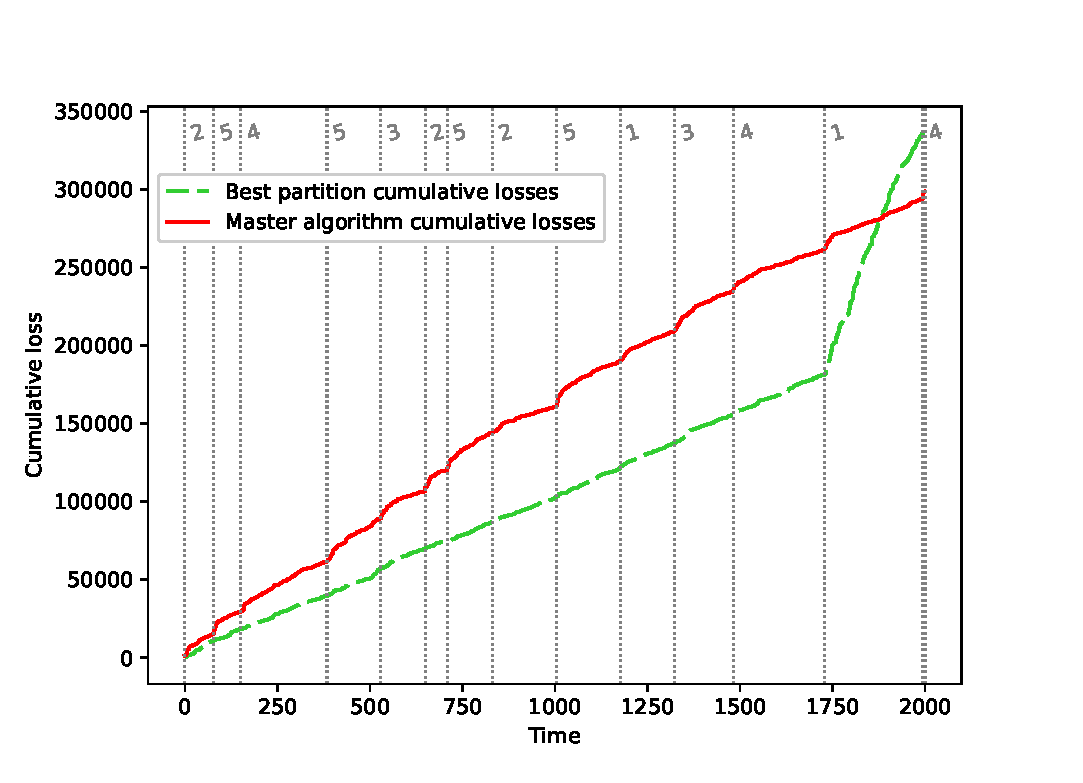
\includegraphics[width=\linewidth]{dec_noise_8}
  \caption{$\sigma^2$ = 8}
  \label{fig:n_8}
\end{subfigure}\hfil % <-- added

%\medskip
\begin{subfigure}{0.5\textwidth}
  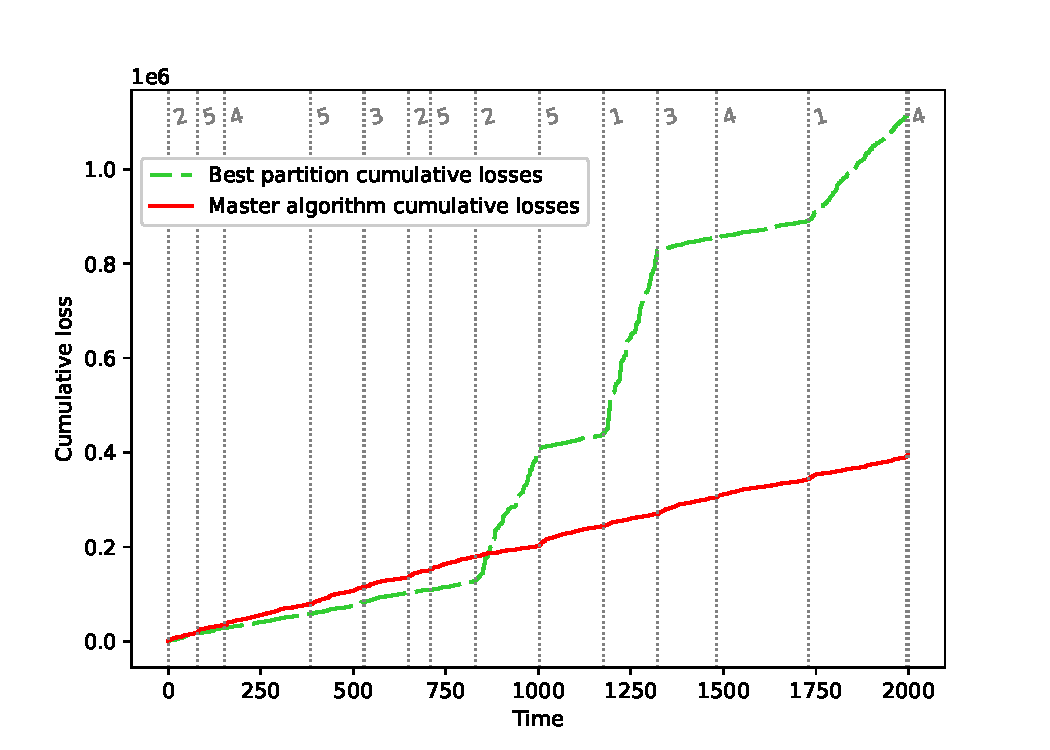
\includegraphics[width=\linewidth]{dec_noise_10}
  \caption{$\sigma^2$ = 10}
  \label{fig:n_10}
\end{subfigure}\hfil % <-- added
\begin{subfigure}{0.49\textwidth}
  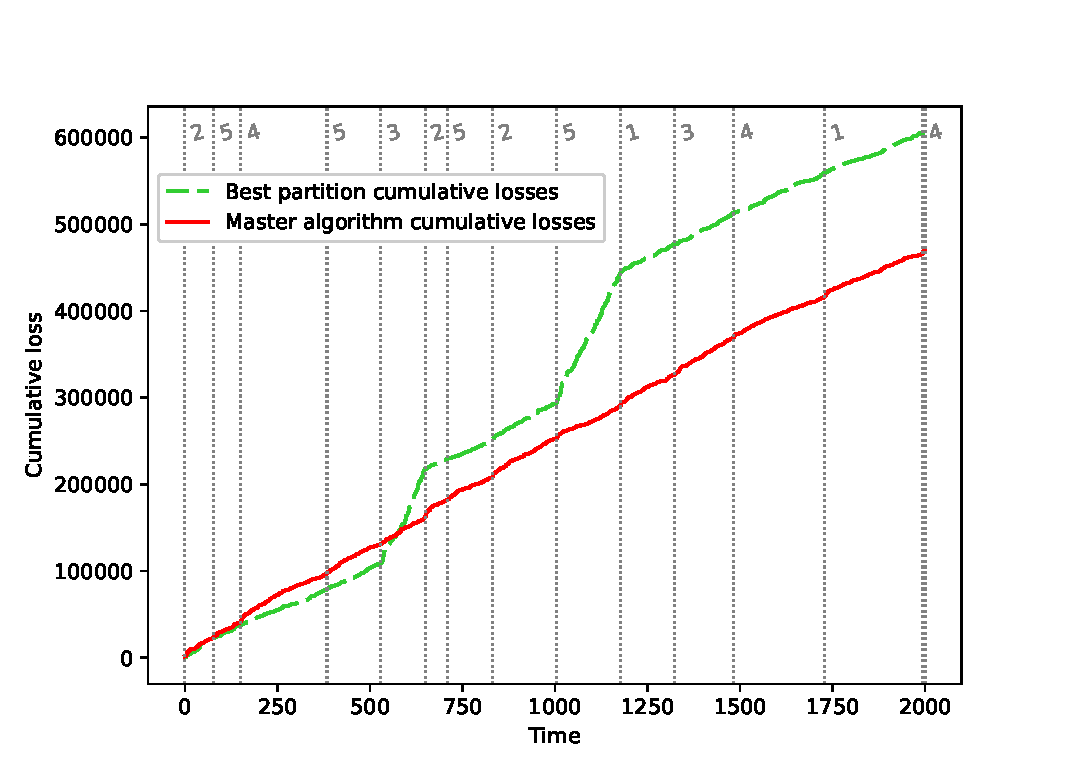
\includegraphics[width=\linewidth]{dec_noise_12}
  \caption{$\sigma^2$ = 12}
  \label{fig:n_12}
\end{subfigure}

\caption{\begin{varwidth}[t]{\linewidth}\centering Total losses with different noise variance $\sigma^2$  (mixing scheme is <<decaying past>>, \\ alpha function is defaut, weight function is $1/x^{1.01}$, window size = 10, random seed = 103)\end{varwidth} \label{fig:noises}}
\end{figure}

\newpage

%--------------------------------------------------------------------------------------------------------------------

\subsection{Impact of Mixing Update Coefficients}

Table \ref{table:diff_af} examines the effect of different coefficients used in the Start Vector Share Mixing Update on the regret. 
The update coefficient controls how much the past weights distribution among experts influences the new distribution versus the current distribution. The table once again confirms that the weights initialization function $1/x^{0.5}$ is the best among others, and shows that with this function, 
the default mixing update coefficient $\alpha_t = 1 / (t + 1)$ stands out as a strong performer, with no serious competitors among other update coefficient functions. 

\begin{table}[H]
\centering
\begin{tabular}{r|cccc}
\toprule
 & \multicolumn{4}{c}{Weight function} \\
\toprule
{Alpha function} &
\centering $\dfrac{1}{{(x+1)\ln^2(x+1)}}$ &
\centering $\dfrac{1}{x^{1.01}}$ &
\centering $\dfrac{1}{x^{0.5}}$ &
\centering $\dfrac{1}{c}$ 
\tabularnewline
\midrule
$1 / (t + 1)$ & 175594.64 & 132268.30 & \contour{black}{108630.68} & 113998.26 \\
$1 / (t + 1)^{0.5}$ & 245494.10 & 207099.32 & 164079.31 & 141554.07 \\
$1 / (t + 1)^{1.5}$ & 130339.21 & 125699.71 & 130185.66 & 131329.66 \\
$1 / (t + 1)^2$ & 136029.09 & 134929.54 & 133876.06 & 132709.43 \\
$1 / e^{t/3}$ & 136413.87 & 135409.06 & 134012.15 & 132760.88 \\
$1 / (t + 10)$ & 175411.17 & 132208.09 & \contour{black}{108638.55} & 114051.47 \\
$1 / (t + 100)$ & 173760.98 & 131623.56 & \contour{black}{108732.56} & 114568.90 \\
$1 / (t + 1000)$ & 162129.20 & 127165.47 & \contour{black}{110389.16} & 118512.52 \\
$1 / 100$ & 220008.81 & 163117.40 & 129035.87 & 117521.60 \\
$1 / 500$ & 198094.83 & 141385.79 & 111706.58 & \contour{black}{108969.41} \\
$1 / 1000$ & 184324.73 & 135612.25 & \contour{black}{109449.15} & 111709.95 \\
$1 / 5000$ & 147561.46 & 121905.50 & 115147.43 & 123741.66 \\
$1 / 10000$ & 136414.42 & 119357.81 & 120634.74 & 127510.93 \\
$1 / 50000$ & 130783.65 & 125141.06 & 129963.25 & 131542.49 \\
\bottomrule
\end{tabular}
\caption{\begin{varwidth}[t]{\linewidth}\centering Regret with different Alpha and Weight Functions in Start Vector Share Update scheme  \\($\sigma^2 =1$, window size = 10)\end{varwidth} \label{table:diff_af}}
\end{table}

%--------------------------------------------------------------------------------------------------------------------

\subsection{Gamma parameter in Increasing Past Share Mixing Update}

Table \ref{table:gamma} specifically examines the impact of the $\gamma$ parameter in the <<Increasing Past Share>> mixing scheme. $\gamma$ controls how quickly the weight given to past expert predictions increases. 
The table shows that the impact of the gamma parameter varies depending on the weight function. 
Interestingly, overall the  difference across $\gamma$ is relatively small.

\begin{table}[h]
\centering
\captionsetup{justification=centering}
%\caption{Regret value for different $\gamma$ in Increasing Past Share Mixing Update scheme }
\begin{tabular}{r|cccc}
\toprule
 & \multicolumn{4}{c}{Weight function} \\
\toprule
{$\gamma$} &
\centering $\dfrac{1}{{(x+1)\ln^2(x+1)}}$ &
\centering $\dfrac{1}{x^{1.01}}$ &
\centering $\dfrac{1}{x^{0.5}}$ &
\centering $\dfrac{1}{c}$ 
\tabularnewline
\midrule

$0.5$& 119783.90 & 112279.88 & 118155.78 & \contour{black}{110151.26} \\
$1$ & 122383.91 & 111221.38 & 117241.85 & \contour{black}{110438.09} \\
$2$& 126865.67 & \contour{black}{110089.54} & 116216.44 & 111563.64 \\
$4$ & 133447.69 & \contour{black}{109160.56} & 115299.68 & 113922.30 \\
\bottomrule
\end{tabular}
\caption{\begin{varwidth}[t]{\linewidth}\centering Regret with different $\gamma$ in Increasing Past Share Mixing Update scheme  \\(alpha function is defaut, $\sigma^2 =1$, window size = 10)\end{varwidth} \label{table:gamma}}
\end{table}


%\newpage
%--------------------------------------------------------------------------------------------------------------------

\subsection{Impact of Mixing Scheme}
%

\begin{table}[H]
\centering

\begin{tabular}{c|ccc|ccc}
\toprule
Mixing scheme & \multicolumn{3}{c|}{start} & \multicolumn{3}{c}{increasing past} \\
\midrule
\backslashbox{$\alpha_t$}{$w_1^x$} &
$\dfrac{1}{x^{1.1}}$ &
$\dfrac{1}{x^{0.5}}$ &
$\dfrac{1}{c}$ &
$\dfrac{1}{x^{1.1}}$ &
$\dfrac{1}{x^{0.5}}$ & 
$\dfrac{1}{c}$ \\
\midrule
$1 / (t + 1)$ & 132268 &  \contour{black}{108631} & 113998 & \contour{black}{110438} & 111221 & 117242 \\
$1 / (t + 1)^{0.5}$ & 207099 & 164079 & 141554 & 183749 & 160168 & 145260 \\
$1 / (t + 1)^{1.5}$ & 125700 & 130186 & 131330 & 131002 & 131850 & 131691 \\
$1 / (t + 1)^2$ & 134930 & 133876 & 132709 & 135243 & 133936 & 132722 \\
$1 / \ln(t + 1)$ & 418163 & 340332 & 309672 & 400131 & 337777 & 312109 \\
$1 / e^{t/3}$ & 135409 & 134012 & 132761 & 135409 & 134012 & 132761 \\
$1 / (t + 10)$ & 132208 & \contour{black}{108639} & 114051 & \contour{black}{110259 }& 111266 & 117299 \\
$1 / (t + 100)$ & 131624 &  \contour{black}{108733} & 114569 &  \contour{black}{109744}& 111719 & 117835 \\
$1 / (t + 1000)$ & 127165 & \contour{black}{110389} & 118513 & \contour{black}{110754} & 115362 & 121522 \\
$1 / 100$ & 163117 & 129036 & 117522 & 129874 & 125704 & 120981 \\
$1 / 500$ & 141386 & 111707 &  \contour{black}{108969} & 112134 & \contour{black}{110618} & 112210 \\
$1 / 1000$ & 135612 &  \contour{black}{109449} & 111710 &  \contour{black}{109844} & \contour{black}{110794} & 115281 \\
$1 / 5000$ & 121906 & 115147 & 123742 & 115334 & 121027 & 125928 \\
$1 / 10000$ & 119358 & 120635 & 127511 & 121016 & 125808 & 128881 \\
$1 / 50000$ & 125141 & 129963 & 131542 & 130965 & 131895 & 131885 \\
\bottomrule
\end{tabular}
\caption{\begin{varwidth}[t]{\linewidth}\centering Mean values with different Mixing Update schemes and Weight and Alpha functions  \\($\sigma^2 =1$, window size = 10)\end{varwidth} \label{table:mt} }
\end{table}

\begin{figure}[H]
\centering % <-- added
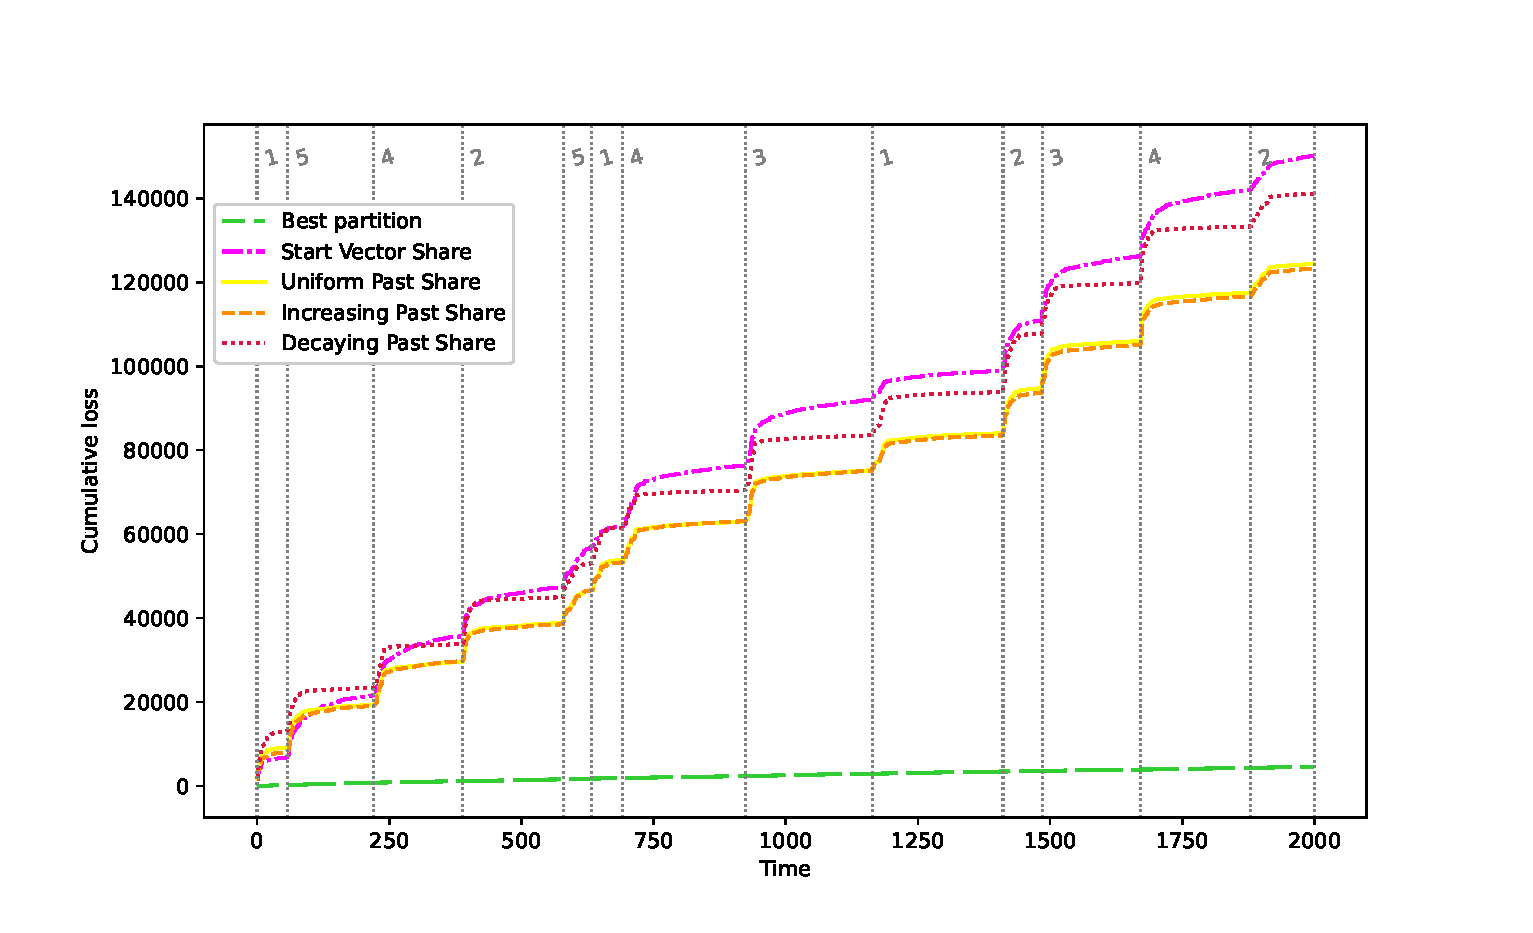
\includegraphics[width=0.9\linewidth]{diff_mt_styled}
\caption{\begin{varwidth}[t]{\linewidth}\centering Total loss with different mixing schemes  \\ (alpha function is defaut, weight function is $1/x^{1.01}$, $\sigma^2 =1$, window size = 10)\end{varwidth} \label{fig:mt}}
%\caption{Total loss for different mixing schemes}
\medskip
\end{figure}


Table \ref{table:mt} focuses on the performance of the <<Start Vector Share>> and <<Increasing Past Share>> mixing schemes with different weight functions and update coefficients. In general, <<Start Vector>>  scheme shows a preference for the $1/x^{0.5}$ weight function, while <<Increasing Past>> works better with the  $1/x^{1.1}$ weight function.
Figure \ref{fig:mt} compares cumulative losses of master algorithm with different mixing shemes.



%--------------------------------------------------------------------------------------------------------------------

\section{Conclusion}

This paper explores the impact of hyperparameters on the GMPP algorithm, an online aggregation method for predicting locally stationary time series using a countable number of experts. The study systematically analyzes the influence of initialization weights, mixing update coefficients, mixing schemes, and expert window size.

Results demonstrate that the optimal choice of hyperparameters depends heavily on the chosen mixing scheme. For instance, the <<Increasing Past Share>> mixing scheme, proposed in this study, shows promising results, particularly when combined with specific weight functions. Interestingly, higher noise levels can lead to lower regret, sometimes even resulting in negative regret, indicating that the algorithm can outperform the best partition in noisy environments.

%In conclusion, this study emphasizes the significant impact of these adjustments on the GMPP algorithm's effectiveness. It highlights the importance of carefully selecting these settings based on the characteristics of the data and the desired performance goals. Further research is encouraged to explore optimal configurations for specific applications.

%
%\section{Preparing a manuscript}
%\noindent
%Manuscripts are prepared using \verb'jmlda.sty' style package.
%You are recommended to use \verb'jmlda_rus.bst' and \verb'jmlda_eng.bst' style files for generating bibliography using Bib\TeX.
%
%Visit the \url{http://jmlda.org/?lang=en} website for detailed submission instructions, templates and other information.
%
%Please note that this file must be saved in~\verb'UTF-8' encoding. Where possible select~\verb'UTF-8 without BOM' encoding. 
%To change the encoding please use \verb'Sublime Text' or \verb'Notepad++' text editors.
%
%\section{Structure of the article}
%\noindent
%Divide your article into clearly defined and numbered sections and paragraphs.

%\section{Concluding Remarks}
%This section should provide the summary and explore the significance of the results achieved and list problems not yet solved.
%Results should be clear and concise.

%%%% please specify doi of the cited item if possible, see~\bibitem{article}
%%%% Crossref doi of the item can be retrieved at http://www.crossref.org/guestquery/
\clearpage
\begin{thebibliography}{99}

\bibitem{article}
    \BibAuthor{V.\,V’yugin, V.\,Trunov}. 2023.
    Prognozirovanie lokal'no statsionarnykh dannykh s ispol'zovaniem predskazanii ekspertnykh strategiy
    [Prediction of Locally Stationary Data Using Prediction with
Expert Advice].
    Available at: \BibUrl{http://www.jip.ru/2023/470-487-2023.pdf}
    
\bibitem{article98}
    \BibAuthor{M.\,Herbster, M.\,Warmuth}. 1998.
    \BibTitle{Tracking the best expert}.
    Available at: \BibUrl{https://link.springer.com/content/pdf/10.1023/A:1007424614876.pdf}
    
\bibitem{article02}
    \BibAuthor{O.\,Bousquet, M.\,Warmuth}. 2002.
    \BibTitle{Tracking a small set of experts by mixing past posteriors}.
    Available at: \BibUrl{https://www.jmlr.org/papers/volume3/bousquet02b/bousquet02b.pdf}


\bibitem{book}
    \BibAuthor{N.\,Cesa-Bianchi, G.\,Lugosi}. 2006.
    \BibTitle{Prediction, Learning, and Games}.
    Available at: \BibUrl{https://ii.uni.wroc.pl/~lukstafi/pmwiki/uploads/AGT/Prediction_Learning_and_Games.pdf}
    
\bibitem{ebook}
    \BibAuthor{Hyndman,\,R.\,J. \& Athanasopoulos,\,G., 2nd edition}. 2018.
    \BibTitle{Forecasting: Principles and Practice}.
    \BibJournal{OTexts: Melbourne, Australia} .
    Available at: \BibUrl{https://otexts.com/fpp2/}
    
    
\bibitem{vvbook}
    \BibAuthor{V.\,V'yugin}. 2022.
    Matematicheskie osnovy mashinnogo obucheniya i prognozirovaniya 
    [Mathematical Foundations of Machine Learning and Forecasting].
    Available at: \BibUrl{http://iitp.ru/upload/publications/6256/vyugin1.pdf}


            
\end{thebibliography}

\end{document}
